\section{Tweedimensionale stapelproblemen}

\subsection{Algemeen}
In de voorbije lessen hebben we het vooral gehad over complete vlakvullingen, i.h.b. het vullen van vlakken met vierkanten. 
In dit onderdeel zullen we kijken naar het vullen van vlakken met figuren die het vlak nooit volledig zullen vullen. We zullen het hebben over tweedimensionale stapelproblemen. We zijn namelijk op weg om het bolstapelprobleem van Kepler te bekijken! 
Bij het stapelen in twee dimensies hebben we minder mogelijkheden dan bij het stapelen in drie dimensies, maar we kunnen er toch heel veel over zeggen. Als we denken aan tweedimensionale stapelingen, dan denken we aan een vlak waarin we voorwerpen stapelen die twee dimensies hebben. Deze voorwerpen kunnen heel uiteenlopend zijn. Wij zullen hier cirkels stapelen, maar je kan evengoed ellipsen, achthoeken ... stapelen. Naar analogon met het bolstapelprobleem van Kepler waarbij we met bollen zullen werken bekijken we het geval van de cirkels. 


In de eerste les hebben we reeds gezien dat je een oneindig vlak volledig kan vullen met identieke gelijkzijdige driehoeken, vierkanten en zeshoeken. Dit noemen we 100\% effici�ntie. 

\textbf{Vraag:} Hebben we ook 100\% effici�ntie als we een oneindig vlak zouden betegelen met cirkels?

Het antwoord is natuurlijk 'neen'. Maar wat is de effici�ntie dan wel? En in welke configuratie is deze het beste?

\begin{opdracht}
Probeer de cirkels (munten, flippo's, pokerjetons ...) eens zodanig op een tafel te leggen dat er zo weinig mogelijk ruimte tussen de cirkels overblijft. 
\end{opdracht}

Het was reeds duidelijk je nooit elk plekje van de tafel kunt bedekken als de cirkels elkaar niet mogen overlappen.
We zijn in eerste instantie ge�ntereseerd in rangschikkingen van oneindig veel cirkels op een oneindige grote tafel. Je hoeft dan geen rekening te houden met wat er aan de randen gebeurt. De randen maken alles moeilijker (maar ook interessanter), daar zullen we verderop naar kijken. E�n voor de hand liggende mogelijkheid om de cirkels zo effici�nt mogelijk in het vlak te rangschikken is om ze netjes naast en boven elkaar te leggen, volgens een patroon van vierkantjes. Dat dit niet de best mogelijke oplossing is wordt al snel duidelijk door wat met de rijen te schuiven. Je kunt de rijen namelijk iets beter in elkaar laten passen. Iedere cirkel raakt dan aan zes andere cirkels \todo{Vermelden van kissingnumber?}, in plaats van aan vier, zoals in het vierkante geval. De cirkels komen nu in een regelmatig patroon te liggen op een zogenaamd hexagonaal rooster. Het lijkt onmogelijk om de cirkels nog dichter bij elkaar te krijgen. Dat dit inderdaad niet beter kan werd ongeveer honderd jaar geleden bewezen door de Deense getaltheoreticus Thue. Een schets van het bewijs zullen we zo meteen bekijken. Eerst gaan wij zelf op zoek naar wat nu juist de effici�ntie is en hoe je deze moet berekenen.

\subsection{Voronoicellen}

Om te berekenen hoe effici�nt een rangschikking met cirkels is, maken we gebruik van Voronoicellen. De Voronoicel van een cirkel is de verzameling van alle punten die dichter bij het middelpunt van deze cirkel liggen dan bij het middelpunt van een andere cirkel, alle punten dus die het dichtst bij d�t middelpunt liggen. 

\textbf{Vraag:} Hoe ziet de Voronoicel eruit bij een vierkante rangschikking? Hoe ziet de Voronoicel eruit bij de hexagonale rangschikking?
\answer{Bij de vierkante rangschikking is zo'n Voronoicel een vierkant dat strak om de cirkel zit, en voor de hexagonale rangschikking is het een regelmatige zeshoek.}

\textbf{Vraag:} Hoe kan je de effici�ntie berekenen aan de hand van zo'n Voronoicel?
\answer{Het percentage van het vlak dat wordt bedekt door cirkels is gelijk aan het percentage van de Voronoicel dat door ��n cirkel wordt bedekt, want voor alle cirkels is de vorm van de Voronoicel hetzelfde en de Voronoicellen betegelen samen het hele vlak.}

\todo{Foto: zelf trekken van de jetons!!}

\begin{opdracht}
Bereken voor de vierkante en de hexagonale rangschikking de effici�ntie.
\end{opdracht}
\answer[4cm]{
\begin{enumerate}
	\item \textbf{Vierkante rangschikking}:\\
	Als je cirkels neemt met straal gelijk aan 1, dan heeft het strakke 'omgeschreven' vierkant in de vierkante betegeling een zijde met lengte 2. De oppervlakte van de cirkel hier is $\pi$, de oppervlakte van het vierkant is 4. (Uiteraard konden we andere afmetingen genomen hebben, maar de verhoudingen blijven steeds hetzelfde.) Er is dus $\frac{\pi}{4}=0,78538...$, of ruim 78\% van het totale vlak bedekt door de cirkels.
	\item \textbf{Hexagonale rangschikking}:\\
	De zeshoek om een cirkel met straal 1 kan worden opgedeeld in twaalf halve gelijkzijdige driehoekjes met een basis met lengte 1 en een hoogte van $\frac{1}{\sqrt{3}}$. De oppervlakte van de zeshoek is dus $12.\frac{1}{2}.1.\frac{1}{\sqrt{3}}=2\sqrt{3}$. De effici�ntie of bedekkingsgraad is dus $\frac{\pi}{\sqrt{12}}=0.906589$.
\end{enumerate}}

\subsection{Axel Thue}
De Scandinavische wiskundige Axel Thue (1863-1922) ontwikkelde in 1892 een theorie over het tweedimensionale equivalent voor 'het probleem van Kepler' waarin men zocht naar de dichtste pakkingsmethode voor cirkels in het vlak. Thue betegelde het vlak met identieke gelijkzijdige zeshoeken en tekende in elke zeshoek een cirkel op zo'n manier dat elke cirkel alle zijden van de zeshoek raakte. Hierdoor verkreeg hij een dichtheid van 90.69\%, waarvan hij beweerde dat dit de hoogst mogelijke dichtheid was bij het stapelen in 2 dimensies. 
Om dit te bewijzen tekende Thue een begrensd aantal cirkels met straal 1 die elkaar niet overlapten. Daarna verdeelde hij willekeurig het tweedimensionale vlak in bepaalde gebieden waarbij hij aantoonde dat de dichtheid in elk gebied maximum 90.69\% is. Hierdoor bestond er geen tweedimensionale pakking waarbij de dichtheid groter is dan 90.69\% en op die manier bewees Thue zijn vermoeden dat de hexagonale pakking de dichtste pakkingsmethode was in twee dimensies.
Het volledige bewijs zullen we hier niet meer bespreken, maar we zullen wel even kijken hoe Thue het vlak waarin de cirkels liggen heeft opgedeeld in verschillende gebieden. Hiervoor zullen we een korte vertaling geven van een deel van het oorspronkelijke Engelstalige bewijs dat geschreven is door Axel Thue.

\begin{quotation}
``Teken een grotere cirkel met straal $\frac{2}{\sqrt{3}}$ rond elke cirkel (zie figuur \ref{2D1}). Telkens als twee van deze grote cirkels elkaar snijden, teken je het lijnstuk tussen de twee snijpunten, waarna je twee congruente driehoeken construeert met het lijnstuk als basis en de tophoeken in het centrum van de cirkels (zie figuur \ref{2D2}). Er zal nooit een punt zijn dat tegelijk binnen alle drie de cirkels ligt. Zoals we merken in figuur \ref{2D3} zullen drie grote cirkels elkaar maximum in ��n punt snijden, het cirkelcentrum, als de centra van de drie grote cirkels de tophoeken zijn van een gelijkzijdige driehoek met zijde 2. \\
Dit geeft ons de verdeling van de ruimte: gebieden buiten de grote cirkels (wit), de gelijkbenige driehoeken (groenachtig blauw), en het gedeelte binnen de grote cirkels, maar buiten de driehoeken (lichtpaars) (zie figuur \ref{2D4}).''
\end{quotation}


\begin{figure}[h]
  \centering
  \subfloat[]{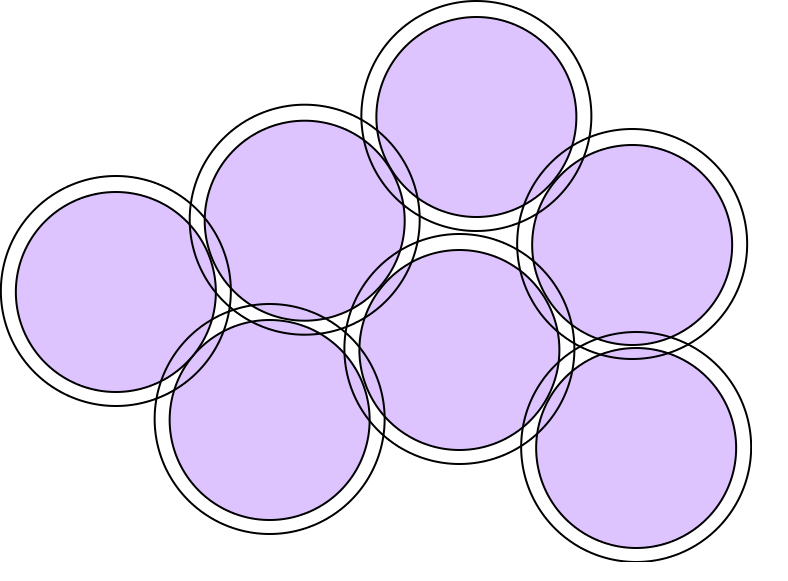
\includegraphics[height=3cm]{2D1}\label{2D1}}
  \subfloat[]{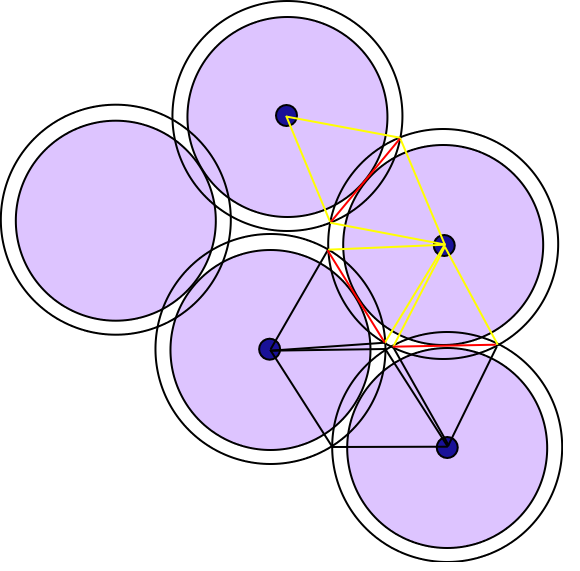
\includegraphics[height=3cm]{2D2}\label{2D2}}\\
  \subfloat[]{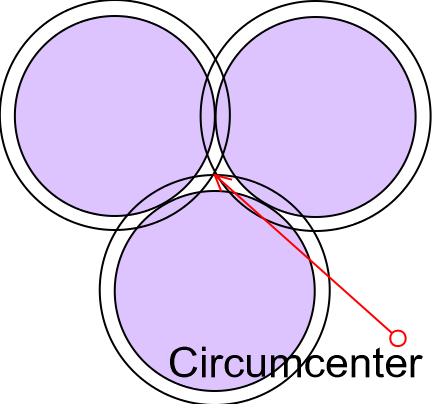
\includegraphics[height=3cm]{2D3}\label{2D3}}
  \subfloat[]{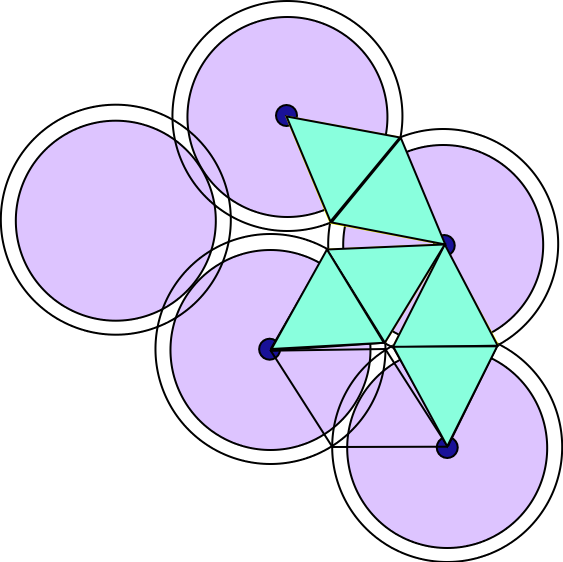
\includegraphics[height=3cm]{2D4}\label{2D4}}\\
  \caption{Figuren bij bewijs van Axel Thue}  
\end{figure}

Uit deze vertaling concluderen we dus dat Thue zijn vlak in 3 gebieden opgedeeld heeft. Hierna zal hij nog berekenen hoeveel oppervlakte er in de drie gebieden wordt ingenomen door de cirkels en uiteindelijk zal hij tot de conclusie komen dat geen enkel gebied een dichtheid heeft van meer dan 90.69\%, waardoor het bewijs voor het tweedimensionale equivalent van het bolstapelprobleem is afgerond.

